% -*-coding: utf-8 -*-

% Vývoj GPU
% Programovací prostředí
    % CUDA
% Architektura GPU (NVIDIA)
    % Hierarchie paměti
    % Hierarchie paralelizace


%čím rychlejší chceme výpočty, tím více omezneí musíme splnit

%Zatím to vypadá, že klasické qsorty atd. budou mít velké overheady
%Zkusit qsort po warpech a porovnat s tím O(n2), co mám teď, ten taky zjemnit na warpy
%Obecně naplnit sdílenou paměť, něco jako pár threadů na pixel

%    -- je to porovnání s 350 na jeden krok VS porovnání s 32 v jednom z několika kroků + scan sumy

%BES na CPU (rozkrájený quickselect)

V této kapitole se stručně seznámíme s historií a vývojem v oboru výpočtů na GPU, rozebereme vlastnosti, přednosti a nevýhody GPU architektury v porovnání s klasickým CPU a nakonec popíšeme programovací model CUDA\footnote{Compute Unified Device Architecture} od společnosti Nvidia, který použijeme pro implementaci filtrů na GPU.

\section{Vývoj GPU}

    kolik sem dát historie? Už to považovat za zajetý obor, nebo zmiňovat celý vývoj? -- Zhruba odstaveček na vývoj od grafického API až po CUDA

    S použitím GPU pro jiné, než grafické výpočty se začalo experimentovat, jakmile přestaly být grafické karty -- hlavně díky rozvoji herního průmyslu -- pouhým jednoúčelovým zařízením a staly se z nich (alespoň částečně) programovatelné paralelní procesory. Vzhledem k tomu, že karty byly primárně ke zpracování grafiky, daly se výpočty provádět pouze pomocí grafického API například přes textury a programovatelné pixel-shadery, což značně snižovalo efektivitu zpracování díky vysoké režii API.

    Zřejmě první \note{(?)} velká společnost, která se rozhodla vyjít vstříc požadavkům na konstrukci GPU jako univerzálně použitelné vysoce paralelní výpočetní jednotky byla Nvidia, když uprostřed vývoje nového čipu\note{ zjistit jakého} změnila celý jeho kocept a zavedla tzv. CUDA-jádra. V únoru 2007 pak představila první verzi vývojového nástroje CUDA (tehdy pouze pro Windows), který umožňoval efektivně využívat hardware GPU pomocí několika rozšíření jazyka C a posléze \Cpp. CUDA-jádra dokonce umí počítat nativně v dvojnásobné přesnosti; u běžných karet jsou ale tři čtvrtiny jader pro dvojitou přesnost deaktivovány (pro grafické operace nejsou třeba), a pro plný výkon ve dvojité přesnosti si musíme koupit (řádově dražší) kartu ze série TESLA, která je primárně určena pro složité výpočty. Veškerý vývojový software poskytuje Nvidia zdarma.

    V současnosti existují k CUDA dvě alternativy: prostředí OpenCL\footnote{Open Compute Language}, zaštítěné sdružením Khronos Group, které se profiluje jako standard pro heterogenní paralelní programování a DirectCompute od Microsoftu stojící na balíku DirectX verze 10 a vyšší. Výhodou OpenCL je, že stejný kód lze zkompilovat jak pro CPU, tak pro GPU výrobců ATI a Nvidia\footnote{jinak se bohužel jedná o vzájemně nekompatibilní technologie}. Z principu tedy nemůže poskytovat tak pohodlný přístup, jako CUDA a výsledkem je poměrně rozsáhlý kód. Dále se tedy budeme zabývat pouze prostředím CUDA a hardwarem s ním souvisejícím.

    \note{jak moc srovnávat? uvést nejnovější karty?}

    \subsection{Současnost}

     Hlavní trend vývoje GPU je nyní v odstraňování omezení, která musíme na kód klást, abychom dosáhli optimálního výkonu a tím pádem se i rozšiřuje množina úkolů vhodných pro zpracování na GPU. Jednotlivé výpočetní jednotky na kartách už dávno nejsou pouhými jednoduchými vektorovými procesory, ale stále více se blíží plnohodnotnému (vícejádrovému) procesoru, i když si samozřejmě svůj vektorový charakter zachovávají. Asi nejvíce je to vidět na práci s pamětí, kde u nejnovějšího čipu \FERMI z dílny Nvidia přibyla vrstva chache, čímž došlo k rozvolnění přístupu do (největší) globální paměti, ale došlo i k rozdělení vektorového procesoru na dva samostatné díly.

\section{Architektura GPU}

    \subsection{Rozdíly CPU a GPU}

        Nyní se podrobněji podíváme na specifika architektury čipů grafických karet. Hlavní otázkou je, pro jaké úlohy jsou vůbec GPU vhodné. Obrázek~\ref{cpu vs gpu} zhruba ukazuje, jak velká část čipu (DRAM ovšem není přímo na čipu) je dedikována pro určitý druh operací.

        \begin{figure}[h]\label{cpu vs gpu}
          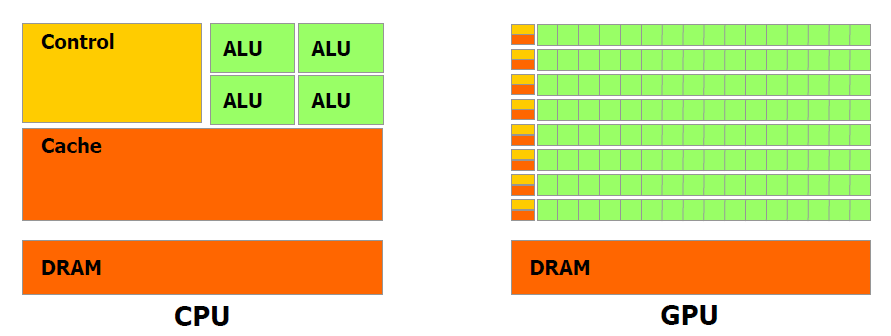
\includegraphics[width = \textwidth]{src/2Gpu/CPUGPU.png}
          \caption{Rozdíly využití čipu na CPU a GPU}
        \end{figure}

        Vidíme, že velkou část čipu CPU zabírá cache a kontrolní logika. Ty zajišťují několika ALU\footnote{Arithmetic Logic Unit} dostatečný přísun dat a instrukcí (např. pomocí hyper-threadingu a branch-prediction), lhostejno jak moc se program větví, nebo jak jsou data uspořádána v DRAM. Naproti tomu GPU se skládá z několika samostatně funkčních vektorových procesorů -- tzv. SM\footnote{Streaming Multiprocesor} jednotek, z nichž každá má vlastní (o několik řádů) menší cache a z kontrolní logiky má naprosté minimum. Z toho plyne jednak jistá nutná disciplína při přístupu do DRAM, která je ale narozdíl od té na CPU lépe optimalizovaná na sekvenční čtení, a za druhé musíme běh programu přizpůsobit tomu, že GPU je po částech SIMD\footnote{Single Instruction Multiple Data}, respektive SIMT\footnote{Single Instruction Multiple Thread -- název pocházející od Nvidia} -- narozdíl od vícejádrového CPU, které je plnohodnotné MIMD\footnote{Multiple Instruction Multiple Data}. Podrobný popis nejnovějšího SM z čipu \FERMI lze nalézt v \cite{Fermi}.
        
        Obecně můžeme říci (protože velká část čipu GPU je dedikována pro aritmetiku), že GPU je nejvíce vhodná pro aritmeticky husté výpočty, tzn. mající vysoký poměr počtu aritmetických operací ku počtu přístupů do paměti. 
        
    \subsection{Algoritmy vhodné pro GPU}
    
        Před paralelizací algoritmu pro GPU musíme tedy zvážit, zda to má vůbec smysl -- pro dosažení optimálního urychlení musí algoritmus v co největší míře splňovat následující body:
        \begin{itemize}
          \item rozložitelnost výpočtů na nezávislé části, které lze vykonávat paralelně (výsledek jedné nezávisí na výsledku předchozí)
          \item malý počet přístupů do paměti, nejlépe sekvenční/blokové
          \item podobný kód ve všech paralelních částech, minimální a předvídatelné větvení kódu
        \end{itemize}
        
        Jak uvidíme, filtrování obrazu nesplňuje tyto body úplně (např. přístupy do paměti) -- kdyby splňovalo vše, tak se jím nemá příliš cenu zabývat -- ale dostatečně na to, abychom dosáhli použitelných výsledků.
    
\section{Pogramovací model CUDA a jeho HW implementace}

    Pro maximální efektivitu paralelizace vyvinula Nvidia několikavrstvou dobře škálovatelnou strukturu s přímou návazností na svůj hardware. Nejmenší výpočetní jednotkou z pohledu programu je \emph{thread} (vlákno), který fyzicky běží na jednom CUDA-jádře v SM. Thready se sdružují do \emph{thread-bloků}, které běží na celém SM a mohou mít 1D, 2D, nebo 3D strukturu, podle toho jakého charakteru jsou zpracovávaná data. Poslední článek tvoří \emph{grid} běžící na celé GPU obsahjící (zatím) nejvýše 2D strukturu thread-bloků. Z programu pak výpočty spouštíme pomocí volání \emph{kernelu} obsahujícího náš kód, kterému sdělíme v kolika thread-blocích má běžet, jakou mají mít strukturu v gridu, kolik threadů má být uvnitř thread-blocku a jak mají být uspořádány. To umožňuje ten samý kernel spouštět na více různých zařízeních, protože sám hardware rozhoduje, jak jednotlivé výpočetní elementy mezi SM (a posléze CUDA-jádra) rozdistribuuje.
    
    \subsection{Úrovně přístupu}
    
    Na straně uživatele poskytuje Nvidia dvě rozhraní: nízkoúrovňové CUDA Driver API a vysokoúrovňové CUDA runtime API, v soušasnosti ve verzi 4.0. Driver API poskytne uživateli totální kontrolu nad kartou výměnou za složitější a delší kód -- uživatel musí zajistit inicializaci zařízení, přesun dat a funkčních parametrů pro kernel na kartu a přesun a spuštění kernelu samotného\note{ kernel musí být v extra souboru?}. Rozhraní Driver API je v C a funkčně zhruba odpovídá OpenCL. Runtime API je rozšířením C, které umožňuje kernel napsat podobně jako funkci v C a při volání jí speciální syntaxí sdělit, kolik threadů a bloků chceme spustit. O inicializaci a vše ostatní se postará runtime. Nevýhodou Runtime API je, že jeden CPU proces nemůže používat více zařízení \note{a naopak?}, což se ale nové verze snaží vylepšit.
    
    Mixování obou přístupů (např. právě kvůli použití více zařízení) se nedoporučuje, ale v rozumné míře možné je -- pravidla mixování stanovila ale až CUDA 4.0. V kódu používáme výhradně Runtime API, proto se dále budeme zabývat pouze jí.
    
    \subsection{Kernel}
    
    Runtime API nám dovoluje míchat kód pro CPU i GPU v jednom souboru, definici kernelu proto rozlišíme specifikátorem 
    \Vr"\cy{__global__}" (příklad převzat z \cite{CUDA programming g.}).
    
    \begin{Verbatim}[commandchars = \\\{\}]
    // definice kernelu
\cy{__global__} \bl{void} MyVecAdd(\bl{float} *A, \bl{float} *B, \bl{float} *C)\{
    \bl{int} i = \cy{threadIdx}.x;
    C[i] = A[i] + B[i];
\}
    // volání kernelu v programu
    MyVecAdd<<<1,N>>>(A,B,C);
    \end{Verbatim}

    Při volání v příkladu specikujeme, že chceme jeden thread-blok a N threadů jako vektor, vektory A, B a C musí být při volání již připraveny v paměti karty. Po spuštění dostane každý thread (potažmo thread-blok) své ID, které je v kódu přístupné skrze read-only proměnnou \Vr"\cy{threadIdx}" (potažmo \Vr"\cy{blockIdx}") a umožní tak diferenciaci threadů.
    
    \subsection{Práce s pamětí}
    
    Jak jsem zmínili v úvodu kapitoly, paměťové zdroje karet jsou poměrně omezené a vhodné zacházení s pamětí je tak prvním předpokladem pro to, aby paralelizovaný algoritmus dosáhl optimálních výsledků. Vývoj jde ale v této oblasti hodně dopředu a architektura FERMI má již paměti mnohem více. V dalším textu budeme tedy uvádět vždy dvě hodnoty



    \subsection{Hierarchie paměti}
    \subsection{Paralelizace instrukcí}


% v implementaci chceme už jen popisovat optimalizace, programming model už musí být hotový 